\subsection{Ej 3: Round-Robin Implementación}
-Explicar la idea y la funcionalidad de c/u de las
estructuras de datos usadas
-Hacer pseudocódigo

\subsection{Ej 4: Round-Robin Simulaciones}

!Explicar por qué: 
-elegimos 1 costo cambio de contexto y 2 costo cambio de nucleo (hay una lista para todos los nucleos)
-es efectivamente un RR
-no siempre es mejor tener más núcleos en un RR con lista global
Esto depende de cuándo entren las tareas, que procesadores
estaban libres y el quantum de c/u

En estas im todos los cpu tienen quantum = 4
-Hacer otros experimentos con dif quantums y ver cuál queda mejor

\begin{center}
 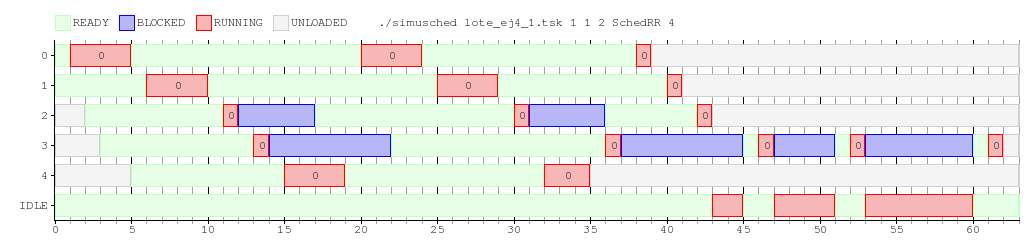
\includegraphics[scale=0.5]{./ej3y4/ej4_1cpu.png}
 % ej4_1cpu.png: 1027x247 pixel, 72dpi, 36.23x8.71 cm, bb=0 0 1027 247
\end{center}

\begin{center}
 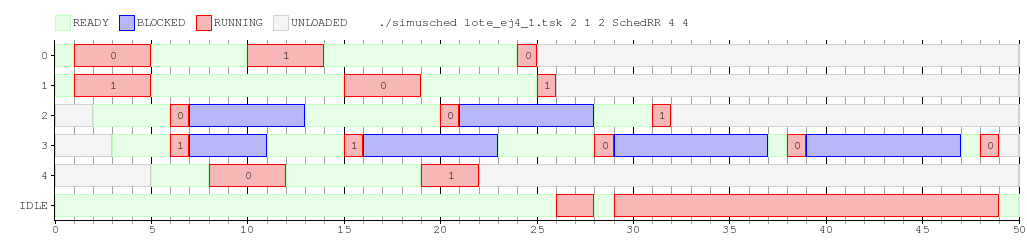
\includegraphics[scale=0.5]{./ej3y4/ej4_2cpu.png}
 % ej4_2cpu.png: 1027x247 pixel, 72dpi, 36.23x8.71 cm, bb=0 0 1027 247
\end{center}

\begin{center}
 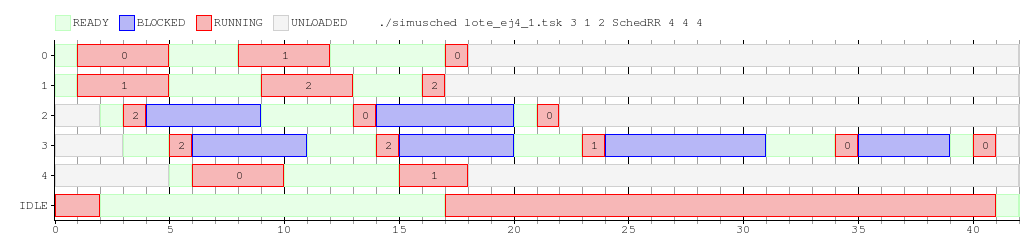
\includegraphics[scale=0.5]{./ej3y4/ej4_3cpu.png}
 % ej4_3cpu.png: 1027x247 pixel, 72dpi, 36.23x8.71 cm, bb=0 0 1027 247
\end{center}

